\chapter{Background and Related Work}\label{ch:background-and-related-work}

While Virtual Reality technology has gained more and more traction over the recent years, 30\% to 80\% of users
encounter some form of sickness symptoms during exposure to virtual reality environments~\cite{Rebenitsch2016}.
Additionally, these sickness symptoms not only occur during the exposure to virtual environments, but can have lasting
effects and affect users after the exposure as well~\cite{LaViola2000}.
The high number of affected users has led to cybersickness being one of, if not the biggest roadblock to a more
widespread adoption of Virtual Reality Devices.

According to LaViola~\cite{LaViola2000} the symptoms of exposure to virtual environments include:
\begin{itemize}
    \item Eye strain
    \item Headache
    \item Pallor
    \item Sweating
    \item Dryness of mouth
    \item Fullness of stomach
    \item Disorientation
    \item Vertigo
    \item Nausea
    \item Vomiting.
\end{itemize}
Vertigo, in the case of VR-sickness particularly benign paroxysmal positional vertigo (BPPV), is a condition where the
individual experiences a false sense of motion, or spinning and objects or surroundings appear to swirl or move~\cite{Post2010}.
\\
Several studies also found that severity of symptoms increases with longer exposure times to virtual environments~\cite{Ruddle2004,Min2004,Duzmanska2018}.
However, some studies show that users can adapt, and overall sickness reduces with repeated exposure~\cite{Hill2000}.

Throughout the study of these symptoms, several terms have been used to compound these sickness symptoms that appear
to be similar to the symptoms of motion sickness.
Initially, the term Simulator Sickness was used to describe motion sickness encountered during exposure to flight
simulators, and originated from the assessment of military flight simulators~\cite{Saredakis2020, Kennedy1993}.
While Simulator Sickness is still used in recent publications, the terms Cybersickness or VR Sickness are generally used
to differentiate from simulator sickness and closer examine the side effects resulting from the use of virtual
environments~\cite{Saredakis2020,McCauley1992}.
The term VR Sickness specifically is used in discussions and studies about sickness symptoms involving head-mounted
displays (HMD)~\cite{Kim2018,Cobb1999}.
This terminology is often used interchangeably across literature.
The terms Cybersickness and VR Sickness will be used in this study, as Stanney, Kennedy, and
Drexler~\cite{Stanney1997} argue that, while sickness from virtual environments shares many of the symptoms often also
experienced during simulator sickness or motion sickness, the sickness profiles are different.
\begin{center}
    \begin{tabular}{ l l l l l}
        \toprule
        \textbf{ } & \textbf{Simulator sickness} & \textbf{Sea sickness} & \textbf{Space sickness} &
        \textbf{Cybersickness} \\
        \midrule
        Highest rating & Oculomotor & Nauseagenic & Nauseagenic & Disorientation \\
        Middle rating & Nauseagenic & Oculomotor & Disorientation & Nauseagenic \\
        Lowest rating & Disorientation & Disorientation & Oculomotor & Oculomotor \\
        \bottomrule
    \end{tabular}
    \captionof{table}{Related conditions symptom profiles according to Rebenitsch and Owen~\cite{Rebenitsch2016}.}
    \label{tab:symptom-profiles}
\end{center}
According to Rebenitsch and Owen~\cite{Rebenitsch2016} cybersickness and other sickness symptoms similar to motion
sickness are polysymptomatic (many symptoms) and polygenic (different manifestation for individuals) and therefore
complex to understand and describe.
To make the sickness and its symptoms easier to survey and examine, Kennedy et al.~\cite{Kennedy1993} categorize the
symptoms listed above into three categories:
\begin{itemize}
    \item Nauseagenic symptoms (dryness of mouth, fullness of stomach, nausea, etc.)
    \item Oculomotor sypmtoms (eye strain, headache, etc.)
    \item Disorientation symptoms (vertigo, dizziness, etc.)
\end{itemize}
The main arguments for the distinction between simulator sickness and cybersickness are that during cybersickness,
disorientation symptoms rank highest and oculomotor symptoms rank lowest, while simulator sickness and traditional
motion sickness usually have the inverted profile, where disorientation symptoms rank lowest~\cite{Stanney1997}.

Cybersickness can also occur without stimulation to the vestibular system, purely through visual cues, unlike motion
and simulator sickness, where stimulation of the vestibular system is needed, but not visual stimulation~\cite{LaViola2000}.
Additionally, Stanney et al.~\cite{Stanney1997} determined that cybersickness can be up to three times more severe
than simulator sickness.
Saredakis et al.~\cite{Saredakis2020} also note significantly higher average Simulator Sickness Questionnaire scores,
although both mention, the scores and questionnaire were established with a focus on military flight simulators used
by military personnel.
While recently, the Simulator Sickness Questionnaire has been adopted to measure cybersickness in virtual
environments, which might be the reason for the higher average scores~\cite{Saredakis2020}.


\section{Common causes of cybersickness}\label{sec:common-causes-of-cybersickness}

Over the recent years there have been several theories trying to explain the sickness symptoms experienced during
extended exposure to virtual environments, especially since the commercialisation of head-mounded virtual reality
devices.
The most common Theories are the sensory conflict theory and the postural instability theory.
Additionally, there are some theories that try to explain why sickness symptoms occur in virtual environments like the
rest frame theory, and the vergence accommodation conflict theory.


\subsection{Sensory conflict theory}\label{subsec:sensory-conflict-theory}

The generally most accepted, and widespread theory is based on a sensory mismatch either between sensory systems of the
body, or between sensory input and expectation given the perceived environment.
Most commonly, a sensory conflict due to vection (the illusion of self movement while stationary) is argued to be the
main cause of cybersickness~\cite{Weech2018,Keshavarz2019}.
Although, other studies like Palmisano, Mursic, and Kim~\cite{Palmisano2017} suggest, that vection is neither the
sole, nor primary source of sensory conflict.
Sensory conflicts like vection can also occur outside virtual environments, for example when a person is in a
stationary vehicle while an adjacent vehicle begins to move~\cite{LaViola2000}.

\begin{figure}[h]
    \centering
    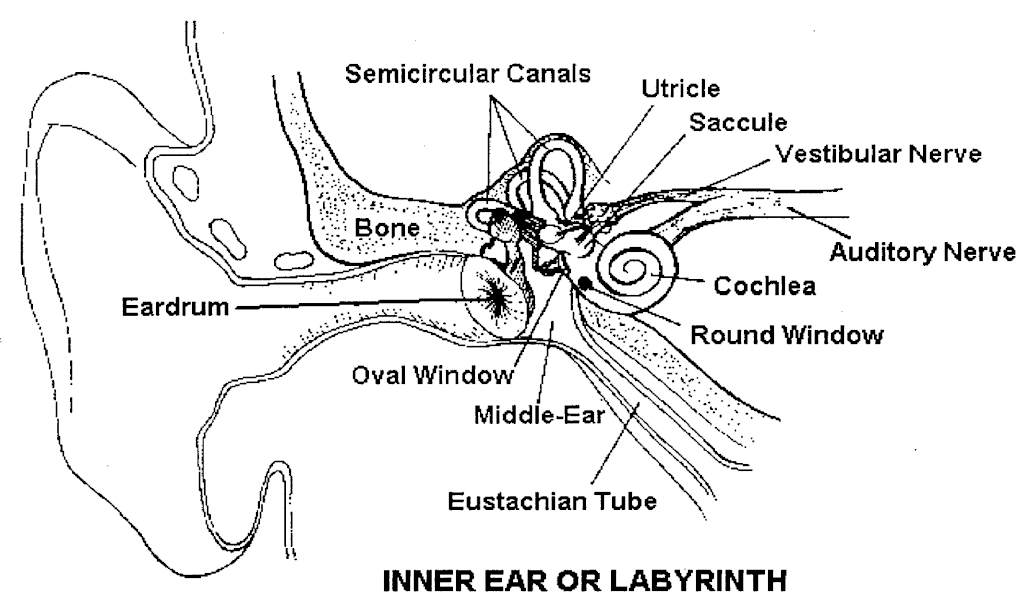
\includegraphics[width=\textwidth]{content/related_work/img/VestibularSystem[LaViola2000]}
    \caption{The components of the vestibular system~\cite{LaViola2000}.}
    \label{fig:vestibular-system}
\end{figure}
Important for the sensory conflict theory are visual perception and the vestibular system, shown in
Figure~\ref{fig:vestibular-system}.
The vestibular system consist of the Semicircular Canals to sense angular momentum, and the Utricle and Saccule to
sense linear momentum.
Together, the system functions to compensate for movement, stabilize vision, maintain head posture, and maintain
balance~\cite{Walker2014}.
In virtual environments, the sensory mismatch is usually between the visual system receiving optical flow patterns
characteristic of self motion, while the vestibular system does not perceive these changes in motion.
This sensory conflict lies at the root of simulator sickness and was identified early on, as Barrett and
Thornton~\cite{Barrett1968} when they noticed that subjects showed symptoms of simulator sickness caused by conflict
between the visual presentation of motion and the lack of corresponding vestibular sensation in their fixed-base
simulators.
Barrett and Thornton also noticed, that subjects only showed sickness symptoms when the simulator was in a
perspective similar to driving a car, but showed no symptoms when viewing the car from outside, similar to driving a
remote controlled car~\cite{Tiiro2018}.

The sensory conflict theory is the most popular theory to explain cybersickness, because it has a lot of studies to
back it up, and is intuitive to understand~\cite{Rebenitsch2016,Tiiro2018}.
However, the theory has been criticised by several studies, because sensory conflict theory only states that sickness
is preceded by a sensory conflict, but the theory is unable to predict when cybersickness will occur, or how severe
sickness symptoms will be~\cite{LaViola2000,Rebenitsch2016,Kolasinski1995}.


\subsection{Postural instability theory}\label{subsec:postural-instability-theory}

Another theory for cybersickness symptoms is the postural instability theory proposed by Riccio and Stoffregen~\cite{Riccio1991}.
They found that motion sickness is preceded by periods of postural instability, where small uncontrolled movements and
changes in the subjects centre of gravity occur, and the subject's ability to maintain postural stability is
hindered~\cite{Riccio1991,Clifton2020}.
Stoffregen and Smart~\cite{Stoffregen1998} translated the theory into three predictions:
\begin{itemize}
    \item Experiences of motion sickness are always preceded by increases in postural instability.
    \item Experiences of motion sickness persist until postural stability is restored.
    \item People who are more naturally unstable are more likely to become motion sick during provocative simulation.
\end{itemize}
These predictions have been solidified and are supported by numerous studies on visually induced motion
sickness~\cite{Clifton2020}.
%%%%%%%%%%%%%%%%%%%%%%%%%%%%%%%%%%%%%%%%%%%%%%%%%%%%%%%%%%%%%%%%%%% add more paper citations here?
Chardonnet, Mirzaei, and Merienne~\cite{Chardonnet2015}, as well as other studies propose to use the changes in 
range, variance, and frequency of the subject's centre of gravity as a measurement of postural sway.
Based on the accessibility of devices to measure individual's centre of gravity, those measurements have found 
increasing popularity in studies to objectively measure postural stability of subjects and indicate the potential 
onset of cybersickness symptoms~\cite{Lim2020}.
\begin{figure}[h]
    \centering
    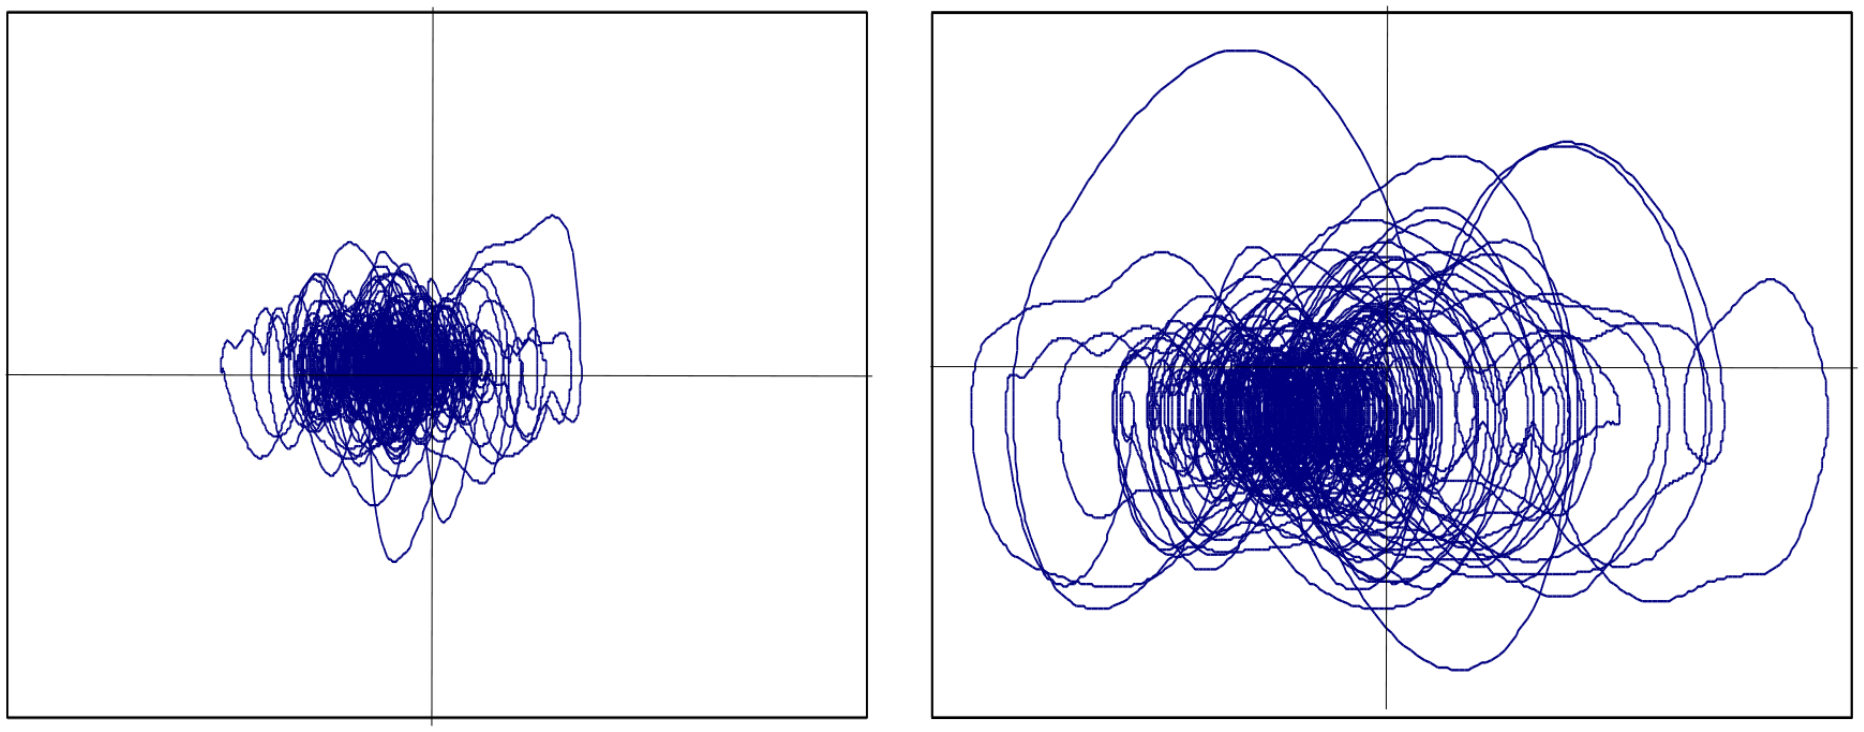
\includegraphics[width=\textwidth]{content/related_work/img/PosturalStability[Smart2013]}
    \caption{Comparison of phase portraits (position (in cm) vs. velocity (in cm/s)) for well (left) and sick (right)
        subjects in a dataset measuring postural stability~\cite{Smart2013}.}
    \label{fig:postural-instability-sample}
\end{figure}
A comparison between the natural postural sway of a subject compared to the postural sway when experiencing motion
sickness is shown in Figure~\ref{fig:postural-instability-sample}.
\begin{figure}[h]
    \centering
    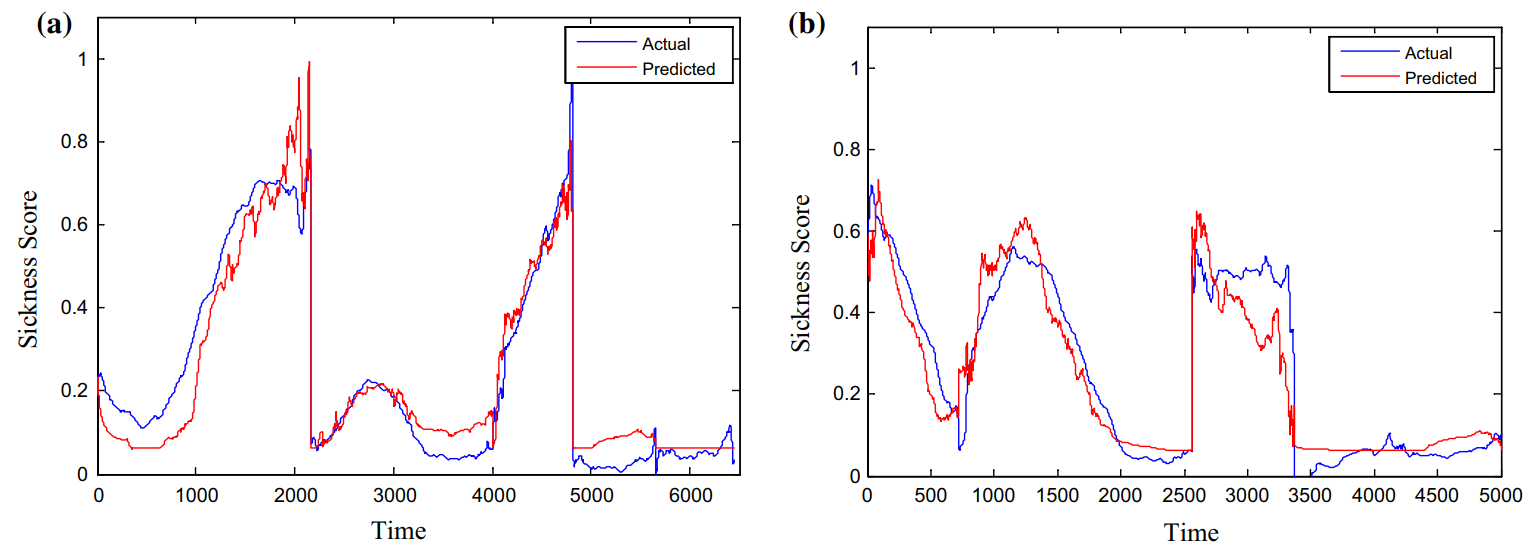
\includegraphics[width=\textwidth]{content/related_work/img/PosturalStabilitySicknessPrediction[Lim2020]}
    \caption{Actual sickness (blue) and predicted sickness (red) of (a) training and (b) testing set produced by the
    prediction algorithm by Lim et al.~\cite{Lim2020}.}
    \label{fig:sickness-prediction-algorithm}
\end{figure}
The recent study by Lim et al.~\cite{Lim2020} successfully used postural stability measurements to train an algorithm
to predict VR content's potential to induce cybersickness, as shown in Figure~\ref{fig:sickness-prediction-algorithm},
based on the postural instability theory.


\subsection{Other theories}\label{subsec:other-theories}

\subsubsection{Rest frame theory}
Similar to sensory conflict theory, the rest frame theory argues that a mismatch in sensed gravitation and perceived
up-direction is the cause for sickness symptoms~\cite{Rebenitsch2016}.
\begin{figure}[h]
    \centering
    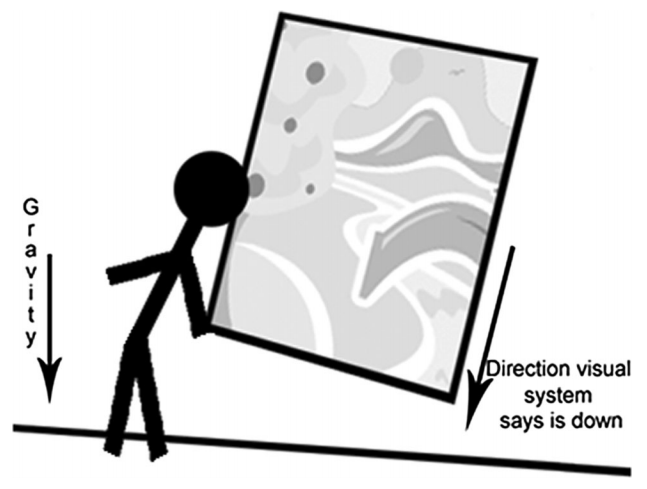
\includegraphics[width=\textwidth/2]{content/related_work/img/SensoryMismatchRestFrame[Rebenitsch2016]}
    \caption{Example of sensory mismatch according to rest frame theory~\cite{Rebenitsch2016}.}
    \label{fig:sensory-mismatch-example}
\end{figure}
An example of this sensory mismatch is shown in Figure~\ref{fig:sensory-mismatch-example}.
Rest frame theory also shows similarities to the postural instability theory, as the discrepancy between the
perceived up-direction and gravity leads to an unstable posture and sickness symptoms following a prolonged period of
postural instability~\cite{Rebenitsch2016}.
The theory also supports the postural instability theory in situations where postural control is lessened, such as in
seated positions where the individual's posture is stabilized.
Several studies like Chang et al.~\cite{Chang2013}, and Duh, Parker, and Furness~\cite{Duh2001b} found, that
superimposing some form of static frame of reference into the virtual environment significantly improves postural
stability and reduces cybersickness symptoms.


\subsubsection{Vergence-accommodation conflict theory}\label{subsubsec:vergence-accommodation-conflict-theory}

Another theory to explain cybersickness symptoms, especially oculomotor symptoms, is the vergence-accommodation
conflict theory.
Vergence is the simultaneous lateral movement of the eyes when an individual's visual system is adjusting to objects
moving towards or away from the individual~\cite{Cassin/Kroeker?}.
%%%%%%%%%%%%%%%%%%%%%%%%%%%%%%%%%%%%%%%%%%%%%%%%%%%%%%%%%%%%%%%%%%%%%%%%%%%%%%%
Accommodation is the process of adjusting both eyes focal lengths to the perceived distance, focusing on the
perceived object~\cite{Rebenitsch2016}.
In virtual environments, especially in head-mounted displays, images are presented at a fixed screen depth.
This leads to a conflict with real life expectations, as vergence and accommodation do not occur naturally in
stereoscopic displays~\cite{Saredakis2020}.
Kim, Kane, and Banks~\cite{Kim2014} noted that content with high levels of stimulation usually contain more changes
in stimulus distance, and therefore not only level of visual stimulation, but also variance of stimulus distance
increase visual discomfort and eye strain.
